\documentclass{article}%
\usepackage[T1]{fontenc}%
\usepackage[utf8]{inputenc}%
\usepackage{lmodern}%
\usepackage{textcomp}%
\usepackage{lastpage}%
\usepackage[head=40pt,margin=0.5in,bottom=0.6in]{geometry}%
\usepackage{graphicx}%
%
\title{\textbf{Gobierno tendrá que indemnizar a Linda Loaiza por violaciones y negligencia}}%
\author{EFE}%
\date{16/11/2018}%
%
\begin{document}%
\normalsize%
\maketitle%
\textbf{URL: }%
http://www.el{-}nacional.com/noticias/politica/gobierno{-}tendra{-}que{-}indemnizar{-}linda{-}loaiza{-}por{-}violaciones{-}negligencia\_260068\newline%
%
\textbf{Periodico: }%
EN, %
ID: %
260068, %
Seccion: %
Política\newline%
%
\textbf{Palabras Claves: }%
Política, Gobierno\newline%
%
\textbf{Derecho: }%
18%
, Otros Derechos: %
1.10%
, Sub Derechos: %
1.10.1%
\newline%
%
\textbf{EP: }%
NO\newline%
\newline%
%
\textbf{\textit{El ente internacional ordenó pagar a la afectada como indemnizaciones compensatorias}}%
\newline%
\newline%
%
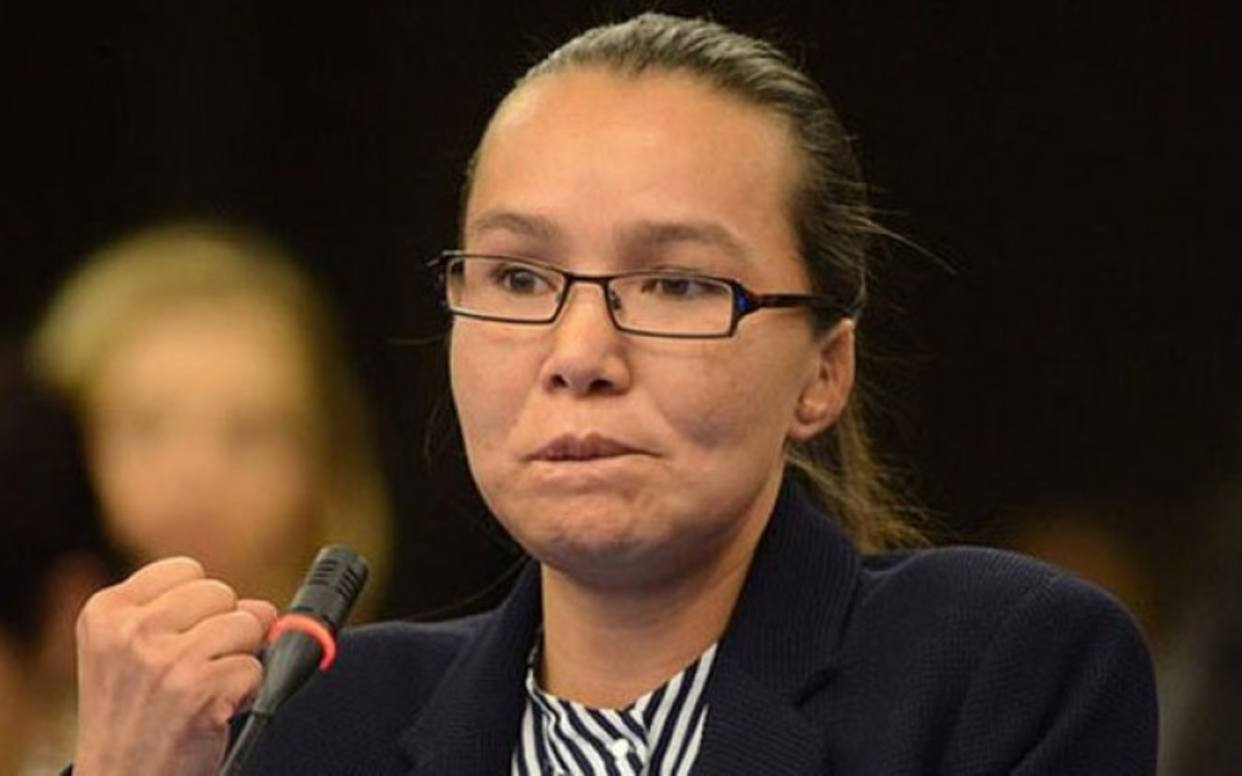
\includegraphics[width=300px]{265.jpg}%
\newline%
%
La Corte Interamericana de Derechos Humanos (CorteIDH) declaró al Estado venezolano como responsable de~una serie de negligencias y violaciones de derechos en el caso de Linda Loaiza López Soto, quien fue secuestrada, torturada, mutilada y violada en 2001.%
\newline%
%
"La Corte Interamericana encontró al Estado responsable por los hechos de tortura y violencia sexual sufridos por Linda Loaiza López Soto, en violación de varias disposiciones de la Convención Americana sobre Derechos Humanos, la Convención Interamericana para prevenir y sancionar la tortura y la Convención Interamericana para Prevenir, Sancionar y Erradicar la Violencia contra la Mujer", explicó el tribunal.%
\newline%
%
El gobierno venezolano tendrá que pagar 30.000 dólares al padre, madre y hermana de Linda Loaiza. 15.000 dólares a otros hermanos, 18.000 dólares a su abogado, además de 25.00 dólares destinados a la organización Cofavic.%
\newline%
%
La joven fue secuestrada por un hombre el 27 de marzo de 2001 cuando tenía 18 años, hasta que, casi cuatro meses después, el 19 de julio de ese año fue rescatada por las autoridades en pésimas condiciones de salud.%
\newline%
%
Lea el documento completo en~CorteIDH%
\newline%
%
\end{document}